\documentclass[a4paper, 10pt, final, garamond]{book}
\usepackage{cours-preambule}

\titleformat{\item}{}{\arabic{item})}{.5em}{}{}
\titleformat{\subitem}{}{\arabic{item}) \alph{subitem} --}{.5em}
{}{}

\makeatletter
\renewcommand{\@chapapp}{Devoir surveill\'e -- num\'ero}
\makeatother

\begin{document}
\setcounter{chapter}{1}

\chapter{Commentaires sur le DS n\degree02}

\section{Commentaires généraux}

Ce deuxième DS est, sous bien des formes, une petite catastrophe. Il faut
prendre le pas sur ce qu'étudier les sciences signifie~: on ne vous demande pas
d'apprendre mais de comprendre. Il faut avoir des bases extrêmement solides pour
bâtir une réflexion digne de ce nom, et absolument éviter les affirmations
choquantes écrites avec certitude.

Votre pratique des DS est à changer radicalement. Il \textbf{faut} lire le sujet
en entier, comprendre où chaque exercice vous emmène, faire des schémas pour
comprendre les situations et intuiter les résultats. Ici, seulement 10 personnes
ont eu plus de 41 points, c'est-à-dire le nombre de points du premier exercice.

Niveau malus, c'est relativement raisonnable. Je note cependant \textbf{trop de
	marges à droite ou absentes}, et des points perdus bêtement par manque d'un
prénom ou d'un numéro de copie. On retrouve surtout des malus d'inhomogénéité.
C'est bien de mettre vos numéros de copie, mais \textbf{ne rendez pas une annexe
	non remplie \textit{et encore moins le sujet}}~!

\begin{tcb}[bld,cnt,fontupper=\Large](impo){Points clés}
	\begin{itemize}
		\item Les interrupteurs, ouverts ou fermés, ne sont PAS des résistances~!
		\item Interrupteur fermé (fil) $\Ra i \neq 0, u = 0$~;
		\item Interrupteur ouvert $\Ra i=0, u \neq 0$~!
		\item Condition initiale $\cancel{\Lra}$ en $t=0$, mais en $t$ initial~!
	\end{itemize}
\end{tcb}

\begin{center}
	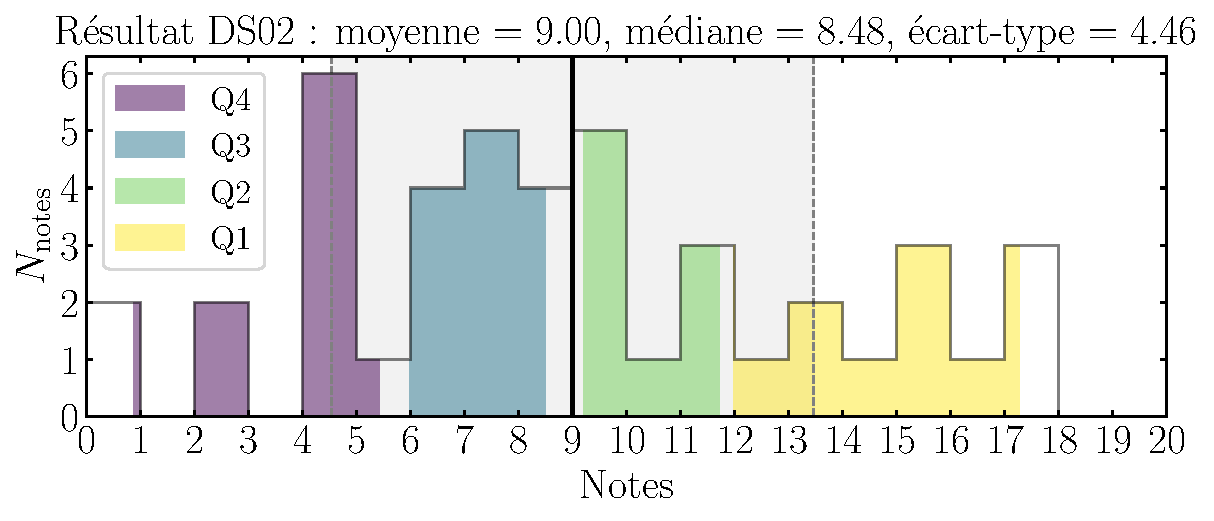
\includegraphics[width=.7\linewidth]{DS02_rslt.pdf}
\end{center}

\setcounter{section}{0}
\exercice[49]{Modélisation d'un dipôle linéaire}
Il manquait les données pour les A.N. Il faut notifier la personne vous
surveillant dans ce cas. Une seule copie en a fait mention écrite, prenez le
réflexe.
\smallbreak
Lisez la consigne~: résultats avec $R$ et $E$ uniquement. \textbf{Nommez vos
	tensions avec précaution~: deux $R$ traversés par des $i$ différents sont des
	tensions différentes~!}

\begin{enumerate}
	\nitem{5} Tout et n'importe quoi. Points pour $R_1+R_2$ en série, $G_1+G_2$ en
	parallèle. Des schémas fantastiques, dans le sens «~créé par l'imagination~».
	\nitem{4} \textbf{Reprenez les exercices sur les résistances équivalentes}.
	Bien essayé pour les court-circuits, mais non.
	\nitem{8} Je vous avais dit de nommer vos points, et qu'un interrupteur ouvert
	a en général une tension non nulle. Aucune débrouillardise pour traiter ce
	circuit en régime permanent.
	\begin{tcb}*(prop)"bomb"{}
		\begin{tasks}(2)
			\task $u = Ri$ ne vaut \textbf{que pour une résistance~!!}
			\task Interrupteur ouvert $\boxed{\Ra u \neq 0}$ par essence~!!
		\end{tasks}
	\end{tcb}
	\nitem{3} 2 bonnes réponses sur 44 copies. \textbf{Ne mettez pas vos tensions
		n'importe où~!!} Une tension est une \textbf{différence de potentiel}, donc
	vous ne pouvez pas simplifier le circuit et dire «~cette tension c'est $v$~».
	\nitem{5} Idem avec les courants. Si vous créez un nouveau nœud, le courant
	représenté n'est plus le même.
	\item[6-8)]{\gpts{13}} RAS.
	\setcounter{enumi}{8}
	\nitem{4} Il faut voir plus loin que la question, et voir le lien avec les
	deux études précédentes.
	\nitem{3} Aucun moyen de faire une résistance équivalente ici. Même
	commentaire, on vous définit $u'$ et $i'$ alimentant une résistance $R_{AB}$…
	\item[11+)]{\gpts{4}} RAS.
\end{enumerate}

\exercice[39]{Point de fonctionnement d'une diode}
\begin{enumerate}
	\nitem{2} Quel dipôle est caractérisé par l'absence de courant le traversant~?
	\nitem{5} Ordonnée à l'origine pas à l'origine, pente en volts, c'était
	n'importe quoi.
	\nitem{2} \textbf{IL SUFFIT DE LIRE LE SENS DES FLÈCHES}~!!! Pas une loi des
	mailles parce que pas de maille.
	\nitem{6} -A, -U, -H, on a tout eu.
	\nitem{5} Refaire le schéma. Il y a une maille. On fait une LdM.
	\nitem{10} Refaire le schéma. On a 3 relations avec $u_D$. On isole.
	\nitem{5} Refaire le schéma. Une maille, un nœud.
	\nitem{4} Pour la seule personne qui est arrivée au bout~: attention, le 0
	n'était pas tout à gauche.
\end{enumerate}

\setcounter{section}{0}
\prblm[45]{Balise lumineuse}
Ce problème est typiquement le genre de sujet où un-e étudiant-e qui a pris la
peine de lire le sujet, de faire un schéma pour comprendre et représenter le
système va mette 15 minutes à commencer mais ira au bout sans embrouille.
\smallbreak
La première question était vraiment cadeau, elle a sauvé 80\% d'entre vous et
vous l'avez bien réalisée d'ailleurs, bravo. Cependant elle est symptomatique de
la différence entre Lycée et CPGE~: en prépa on vous forme à comprendre, pas
apprendre. Vous devez aller plus loin et pouvoir partir d'une
définition pour arriver à un développement nouveau.
\begin{enumerate}
	\nitem{16} \fbox{Résistance infinie $\Ra i=0$} $\Ra$ dipôle équivalent à un
	interrupteur ouvert.
	\nitem{3} Lecture de l'énoncé. \textbf{Attention}, n'appliquez pas $\ln (~)$
	sur des nombres négatifs~! $-\exr^{-t/\tau_1} = \frac{U_a}{E}-1$ ne se passe
	pas au $\ln $, il faut l'appliquer sur $\exr^{-t/\tau_1} = 1 - \frac{U_a}{E} =
		\frac{E-U_a}{E}$. Il faut prendre l'habitude de \textbf{simplifier}~: avoir
	l'expression littérale d'un temps qui commence par $t_a = -\ln (~)$ c'est
	\textit{très} inquiétant puisqu'un temps est positif.
	\nitem{11} Exercice des plus classiques~: RC avec une maille parallèle, donc
	un nœud, donc une LdN. Un peu moins classique, mais clair avec un schéma, la
	condition initale est en $t=t_a$ et n'est pas $E$~!
	\item[4-8)]{\gpts{15}} RAS.
\end{enumerate}

\prblm[84]{Régimes transitoires successifs d'un circuit RL}
Énorme pied de nez à la continuité.
\begin{enumerate}
	\nitem{6} \textbf{NON}, $u$ n'est \textbf{PAS CONTINU} dans un circuit avec
	une bobine~!!! Pour trouver les CI, schéma et LdM.
	\nitem{4} Bobine en RP $\equiv$ fil. LdM.
	\nitem{5} Ne vous précipitez pas, ça n'est pas un RL typique du cours. Il y a
	deux résistances.
	\nitem{8} RAS, TB.
	\nitem{4} Deux choix, comme dans le cours. Une seule bonne réponse.
	\nitem{8} Deux points gratuits pour les asymptotes, mais grosses
	incompréhensions de $\tau$ ou $5\tau$.
	\item[7+)]{\gpts{49}} RAS, pas ou mal traité.
	\item[17-18)] \textbf{Attention}, $\tau$ se trouve à l'intersection
		\textbf{avec l'asymptote}~!!
\end{enumerate}

\end{document}
